The place where the Ground Stations will be placed has to be studied in order to obtain maximum performance of them. This decision will depend mainly on the characteristics of the constellation, the earth topography and the country legislation and resources. In this chapter the analysis and procedures for arriving to the final decision of where the Ground Stations would be placed are exposed.

Given the constellation topology, the coverage of a Ground Station depending on its longitude and latitude will be studied. The aim of this analysis is to show where a Ground Station would have more coverage and give a first approximation and proposal of the 3 Ground Station placement.

\subsubsection{Method}
For the purpose above explained, a Matlab algorithm is developed. This algorithm calculates, on a given moment, how many satellites can be seen from a Ground Station. This calculation will be done several times in order to obtain results along time. In order to elaborate the algorithm the steps showed below are followed:
\begin{enumerate}
\item Calculate where the satellites are referred, using an inertial Cartesian coordinates system, with the origin at the centre of the Earth. This state analysis is done for several time periods with an adequate time-step. 
\item Calculate the Ground Station position referred to the mentioned system. Since the system is inertial, the Ground Station will describe a circle in the rotational plane of the Earth relative to this system. This trajectory depends on the latitude and longitude of where the GS is placed and is calculated for the same time period used before.
\item Calculate, for each time step, how many links can the GS establish. It will depend on the angle between the station and every satellite, and also on the minimum elevation angle. 
\end{enumerate}

Once the algorithm is tested and verified, the links during the day for several longitudes and latitudes and how this parameters affect to the coverage of the station are studied. The code used can be found in \cite[Chapter 1, Section 12]{annex6}, while the study of localisation can be found in \cite[Chapter 3, Section 1]{annex3}.

\subsubsection{Conclusion}
To summarise the results of the analysis, for an optimum performance of every Ground Station, they should be located at latitudes between -62.5º and -57.5º or between +57.5º and +62.5º. For a better performance of the system every Ground Station should be 120º of longitude away of the other GSs if they are at the same latitude or 60º of longitude away if they are at the opposite latitude. Taking in account the topography of the Earth, the following options are proposed (every colour represent the options for one Ground Station):
\begin{figure}[H]
\begin{center}
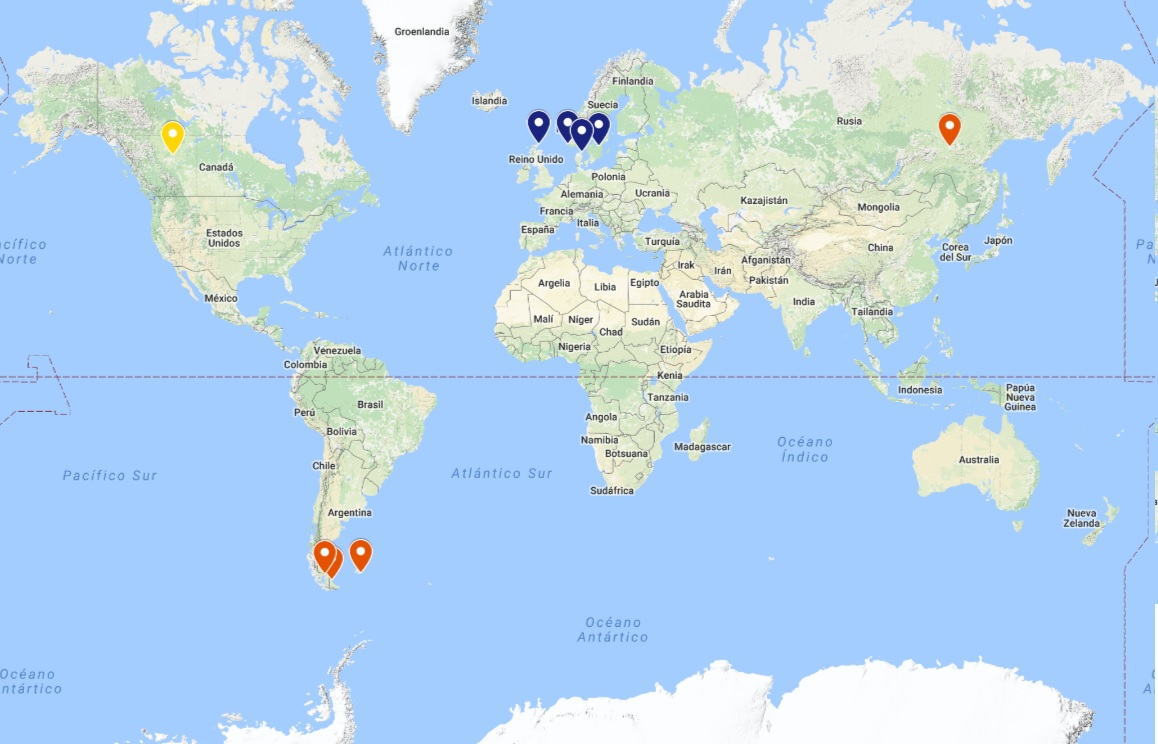
\includegraphics[scale=0.5]{Options.jpg}
\caption{Options for placing the 3 Ground Stations.}
\end{center}
\end{figure}

Given this possibilities a study of the legislation of the involved countries has to be done in order to know the viability of placing there the Ground Stations. The candidate countries, as is shown in the map, are: Canada, Argentina, Chile, Falkland Islands (Islas Malvinas), United Kingdom, Denmark, Norway, Sweden and Russia. 

For the Mission Control Centre, as it does not communicate with any satellite, it has no restrictions on where to build it. It is decided that it will build in Terrassa, since ETSEIAAT is located there and it holds the headquarters of the UPC Space Program.